\chapter{The Main Screen}
\paragraph{Overview}
The Main Screen is the primary display screen. It is shown at power up, and is where Operation Mode (Hand or Automatic) is selected. It displays the Operator Message Centre which provides the Operator with current and relavent machine state information. There are aslo controls for \textit{Automatic \textbf{Cycle Start}} and \textit{Automatic \textbf{Cycle Stop}}, plus \textbf{\textit{Machine Full Stop}}. Finally, there are screen navigation keys provided for Operator access to other machine functions.
\begin{figure}
	\centering
	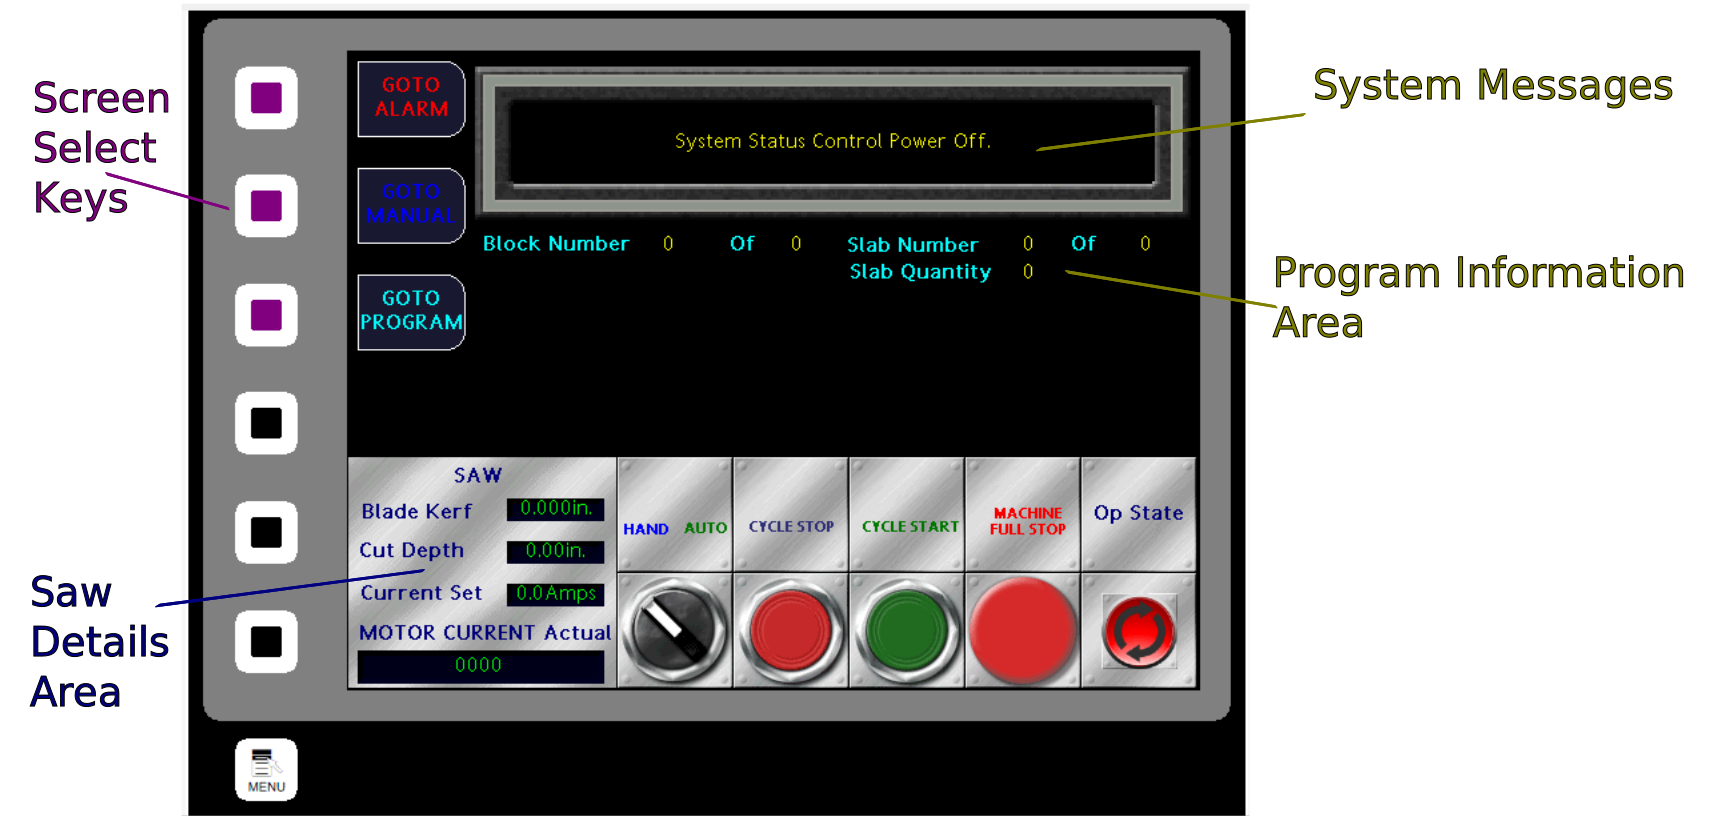
\includegraphics[width=0.5\linewidth]{screen-captures/main-screen}
	\caption{Main Screen}
	\label{fig:main-screen}
\end{figure}
\pagebreak
\paragraph{Main Screen Details}
Main Screen Details are divided into the general categories.
\begin{list}{-}{}
	\item \textbf{Screen Navigation}
	\item \textbf{Operator Message Centre}
	\item \textbf{Saw Information}
	\item \textbf{Program Details}
	\item \textbf{Operation Control}
\end{list}
\paragraph{Screen Navigation}Is performed by using the Programmable Keys (FKeys) located down the left hand side of the OI Terminal. For the Main Screen there are three screens accessible using the labeled FKey's, \textbf{Alarms}, \textbf{Manual}, and \textbf{Program}.
